%&tex
% !TEX program = xelatex
% !TeX TS-program = xelatex
% !BIB TS-program = biber
% !TeX encoding = UTF-8
% !TeX spellcheck = en_US
% !TeX root = ../thesis.tex
%% ==============================
\chapter{Formal Specification-Based Methods}
\label{sec:formal_methods}
%% ==============================

Two of the most important aspects when programming a~\acrshort{acn:plc} are validation and verification.
Validation describes the correctness of the specification compared to the intended use and verification is the correctness of the actual code compared to the specification.
Both aspects ensure that the system behaves as intended.
As~\glspl{acn:plc} are used for real-time applications, the importance of these factors increases even more.
The previously described methods for programming with C offered possibilities in that regard, but they did not improve significantly compared to the IEC 61131-3 languages.
Therefore, in this section the possibilities of using a formal specification to automatically program a PLC are investigated.
This allows to easier validate and verify the developed code.
\citeauthor{Frey:2000aa}~\cite{Frey:2000aa} describe different approaches to verification and validation for~\acrshort{acn:plc} programming.
This paper also gives an overview of different methods that can be used for achieving this.
Based on this overview I investigated the two most used techniques in the following section.

There a several approaches for creating a formal specification of a process or controller~\cite{Frey:2000aa}.
First there are non-model-based approaches that don't require information about the environment or the process for verification.
Approaches employing this method are described in subsection~\ref{sec:non_model}.
Another approach is to use a modeling language to create a model-based specification.
This includes modeling the process environment and the process itself rather than just the behavior.
They also allow for simulation of the system components making evaluation and validation closer to the real-world.
Subsection~\ref{sec:sub:mb} investigates approaches using this specification type.

To compare the different approaches, I look at four criteria that are critical for effective control program development.
For the selection of the comparison criteria I looked at~\cite{VH:2014}.
\citeauthor{VH:2014} compare different model-based PLC programming methods.
From their criteria I selected the four most important ones:
\begin{itemize}
	\item \textbf{Effectiveness} describes the quality and expression strength of the programming method.
	It is determined by the supported programming features, the modularity, the available reuse and the correctness of the model and the transformation.
	Section~\ref{sec:risks} investigates the correctness and the associated risks in more detail.
	\item \textbf{Efficiency} is concerned with the time it takes to create, understand and interact with a model and the generated code.
	This measure is relevant as improved efficiency over traditional programming is one of the key motivations of automated programming approaches.
	\item \textbf{User acceptance} looks at the experience of a developer when using a programming approach.
	Ease of use, required prior knowledge and assistance provided by the approach are key factors here.
	\item \textbf{Real-world applicability} describes the available toolset and integration with existing platforms used in the industry.
	The reasoning behind this is that methods that cannot be employed in a real-world scenario aren't of any use to a developer, even if they excel at other measures.
\end{itemize}

%% ==============================
\subsection{Non-model Based}
\label{sec:non_model}
%% ==============================

Non-model based approaches don't incorporate any knowledge of the actual process but validate the system for all possible input parameters.
This is especially interesting as it allows for a more detailed analysis that is not dependent on assumptions about the process.

For non-model-based methods, I only investigate one formalization method~\acrlong{acn:ltl}, described in~\ref{sec:sub:ltl}.

Another common formalization method for non-model-based approaches are Petri Nets.
A petri net is a bipartite directed graph, that describes an event-transition semantic.
Originally used in mathematics, they were commonly used in the 2000s to model control systems~\cite{Frey:2000:2, Frey:2000aa}.
Modern specification languages incorporate the features of petri nets but use a more user friendly and clear notation.
Therefore they are not elaborated on any further.

%% ==============================
\subsubsection{Linear Temporal Logic}
\label{sec:sub:ltl}
%% ==============================

\acrfull{acn:ltl} is a modal logic that allows to specify behavior over time~\cite{4567924}.
This is done by extending logical operators (and, or, xor, etc.) with temporal operators that specify conditions for the future.
Formally they operate on a sequence of states over the available variables called a Kripke structure.
Common temporal operators are~"\textbf{X}~\textit{A}" (Next), specifying that a formula~\textit{A} is true in the next state,~"\textit{A}~\textbf{U}~\textit{B}" (Until), specifying that~\textit{A} is true until~\textit{B} is true and~"\textbf{G}~\textit{A}", specifying~\textit{A} is true in all states.
With these temporal operators an~\acrshort{acn:ltl} formula can specify a full state graph for different variable changes.
A formula is satisfied by a sequence of states~\textit{S} when its true for all states in sequence.
If a formula is~\textit{valid}, it is satisfied for all possible sequences $ S\in 2^{AP} $ given the set of variables~\textit{AP}.

In this section I will investigate two approaches to automated PLC programming that use~\acrshort{acn:ltl} to validate the specification.

\citeauthor{Kuzmin:2013}~\cite{Kuzmin:2013} use~\acrshort{acn:ltl} to specify the behavior of the controller.
They then use the formulas to verify the specification with a model checker.
Following this the specification is  automatically translated into~\acrshort{acn:ST} code.
In this approach, the variables for the~\acrshort{acn:ltl} are all input variables, output variables and state variables that are used in the PLC program.
For specifying the behavior of the controller, a~\acrfull{acn:ltl} formula defines the change of a variable given a system condition.
To simplify this process, they restrict the values of the variables to Boolean and numerical values and only allow one value change per variable, per PLC working cycle.
\begin{equation}
GX\left(V > \_V \rightarrow OldValCond \land FiringCond \land V := NewValExpr \right)
\label{eq:increase}
\end{equation}
\begin{equation}
GX\left(V > V \rightarrow OldValCond' \land FiringCond' \land V := NewValExpr' \right)
\label{eq:decrease}
\end{equation}
Equation~\ref{eq:increase} shows the proposed~\acrshort{acn:ltl} formula for increasing a variable V given an~\textit{OldValCond} and a~\textit{FiringCond}, equation~\ref{eq:decrease} show the decrease of V.
They define these conditions for all possible alterations of Boolean and numerical values.
The pair of~\acrshort{acn:ltl}s for increasing and decreasing a variable can be translated to a ST program block.
\lstset{language=Pascal}
\begin{lstlisting}[caption={
Auto-generated~\gls{acn:ST} code realizing the~\acrshort{acn:ltl} formulas~\ref{eq:decrease} and~\ref{eq:increase}.~\cite{Kuzmin:2013}},label=lst:ltl:st]
IF OldVarCond AND FiringCond THEN
    V := NewValExpr; (*V+*)
ELSIF OldVarCond' AND FiringCond' THEN
    V := NewValExpr'; (*V-*)
END_IF
\end{lstlisting}
Listing~\ref{lst:ltl:st} shows the~\acrshort{acn:ST} code for the equations~\ref{eq:increase} and~\ref{eq:decrease}.
As the specifications are complex formulas the efficiency of the specification is reduced significantly.
The complex nature makes intensive training and knowledge in modal logic necessary.
This has an adverse impact on the user acceptance and real-world applicability as the specifications are too complex and error prone.
Additionally, they propose a transformation to model checker code that allows to verify the integrity of the model.
This is done by finding a sequence of inputs where one of the LTL formula is not satisfied.
If such a sequence is found, it shows that not all LTL formula a valid, which suggests that the specification is incomplete.
If the LTL formulas are valid, there is no possible state of variables where the program is not acting as specified.
With this method, the verification of the control program is easier as it can be done directly from the specification.
In combination with the substantial number of available constructs in~\acrshort{acn:ltl} formula, this provides a considerable effectiveness.
The only thing missing due to formula-based specification are objects or instances.
Their behavior can be emulated but this requires complex formula constructs.
But the authors don't provide a formal verification of the transformation and argue with the obvious correctness of the transformation.
This full transformation functions and an example can be found in the paper.

The second approach by~\citeauthor{10.1007/978-3-319-74730-9_23}~\cite{10.1007/978-3-319-74730-9_23} uses a~\acrfull{acn:dsl} to describe the control program.
This~\acrshort{acn:dsl} is then validated by transforming it into~\acrshort{acn:ltl} formula and using a model checker.
The actual~\acrshort{acn:plc} code is created by transforming the~\acrshort{acn:dsl} into a~\acrshort{acn:ST} control program.
They use an event \& response semantic for execution so that the system uses controlled transitions to react to unpredictable environment changes.
The~\acrshort{acn:dsl} allows the engineer to specify a scenario-based behavior.
A scenario consists of guarantees, modeling the behavior of the system in each situation, and assumptions, modeling the assumptions an engineer can make on the environment of the system.
An example from the publication~\cite{10.1007/978-3-319-74730-9_23} for a guarantee would be~"\textit{After picking up an item, the feed arm must move to the press, release the item into the press, and finally move back to the feed belt.}" and one of the related assumptions~"\textit{After a robot arm is instructed to pick up an item, it will eventually pick up that item.}.
These guarantees and assumptions can be specified in the~\acrfull{acn:sml}, the~\acrshort{acn:dsl} they use.
They are defined for every output entity to define their reaction to input entities.
Additional keywords for flow control, liveness and safety conditions enable the engineer to give constrains to the specification.
\begin{figure}[h]
	\centering
	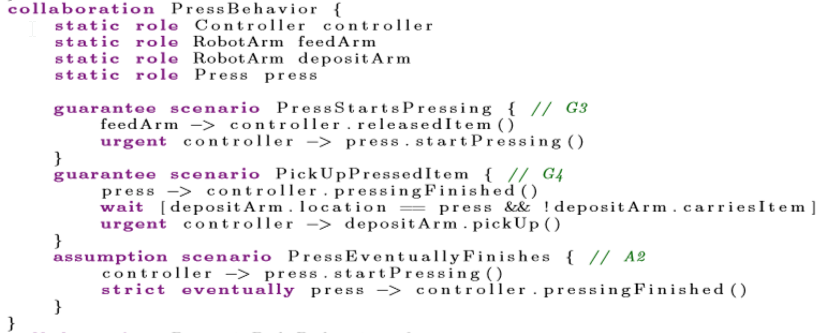
\includegraphics[width=\textwidth]{./Figures/sml_press_beh.png}
	\caption[\acrshort{acn:sml} specification example.]{Example~\acrshort{acn:sml} specification for the behavior of a press.~\cite{10.1007/978-3-319-74730-9_23}}
	\label{fig:sml_press}
\end{figure}
Figure~\ref{fig:sml_press} shows an example of a behavior formalization.
The wait conditions are for flow control and the urgent statements interrupt the current non urgent operation of the controller and prioritize this task.
Such a specification allows for great effectiveness, as most controller scenarios can be covered with it.
The distinct roles and guarantees ease the use of specifying behavior, which allows for better ease of use and efficiency.
They provide an Eclipse based tool named ScenarioTools to create these specifications.
This greatly increases the actual real-world applicability of the approach, as well as the user acceptance due to increased usability and support during development.
The specification is transformed into a game graph, where nodes are the currently active events and the edges are either controllable or uncontrollable input events.
This graph is a game between the controller and the environment, where the controller tries to reach a state with no liveness scenarios and the environment attempts the opposite.
This can be solved with a General Reactivity of rank 1 solving algorithm.
In this GR(1) problem instance, LTL formula with the form
\begin{equation}
\left(\land_{i}\square\diamond a_{i} \right) \rightarrow \left(\land_{i}\square\diamond g_{i} \right)
\end{equation}
must be solved, where $a_{i}$ is assumption i is satisfied and $g_{i}$ is guarantee i is satisfied.
If there is a path through the graph where the assumptions hold true, but the guarantees do not, it's an error in the specification.
This model checking method can be implemented via an~\acrshort{acn:ltl} solver for the transformed GR(1) specification extracted from the~\acrshort{acn:sml} code.
To generate the ST code, this graph is transformed into nested state machines.
Per controller there is a primary state machine modeling the current controller status.
In every possible controller status, there are secondary state machines modeling the uncontrollable input components.
This code generation scheme is beneficial for the efficiency and real-world usability of the approach as the developer can trace changes to the code back to the model and the other way around.
With traceability and maintainability being key factors in industrial applications, this is an important feature.
The authors state that this transformation is valid by design.

\subsection{Model Based}
\label{sec:sub:mb}

Model based specifications use a specification of the controller and a model of the process.
The addition of a process / environment model to the development process allows easier communication and more specific design.
This approach enables a thorough validation and verification.
Commonly simulations and hardware-in-the-loop tests are used to eliminate errors in the early stage of modeling.
In addition, models are often independent of the actual deployment language increasing portability and maintainability over time.
Model-based development is a staple for designing and developing industrial products and plants.

I investigate multiple formalization approaches using model-based specifications to model and define the controller.
They are grouped by the base modeling language used for the specification.
In~\ref{sec:sub:uml}, I look at approaches using~\acrshort{acn:uml} or~\acrlong{acn:sysml}.
\ref{sec:sub:simulink} elaborates on methods using the SIMULINK modeling language.
\ref{sec:sub:grafcet} describes a method using the standardized GRAFCET language.
Lastly,~\ref{sec:sub:plfspecif} looks at the PLCspecif language developed at the CERN.

\subsubsection{UML / SysML}
\label{sec:sub:uml}

\acrfull{acn:uml}~\cite{UML:2-5-1} is a standardized modeling language designed for software engineering.
It defines twelve different diagram types to cover all aspects of system design.
The different diagrams allow different abstraction levels of the system.
For example, use case diagrams are looking at the requirements and use-cases of a system, whereas a class diagram defines the classes that are used to realize a certain functionality.
This makes UML flexible for creating specifications for software systems in different details.

As~\acrshort{acn:uml} is focused on software engineering, the~\acrfull{acn:sysml}~\cite{SysML:1-6} modeling language was created as an adapted subset of~\acrshort{acn:uml}, focused on systems engineering.
Systems engineering focuses on the development of an entire system, composed of multiple components.
It supports the analysis, design, validation and verification of the specification.
Another benefit is the departure from the software centric point of view of UML, that allows SysML to define more broad and complex topics.
For example, regarding embedded development, SysML has extended state machine diagrams allowing to specify more constraints making it usable for defining PLC programs.

In the following section, I am going to look at three approaches that use~\acrshort{acn:uml} or~\acrshort{acn:sysml} to model the system.

\citeauthor{WITSCH2015}~\cite{WITSCH2015, WITSCH20117866} define a subset of the~\acrshort{acn:uml} modeling language called plcML.
This reduces the number of available diagrams to three, allowing for easier definition of PLC behavior.
They use class diagrams for structural modeling and for behavioral modeling, adapted activity and state-machine diagrams.
In addition to this, they provide a code generator for IEC 61131-3 languages.
\citeauthor{Obermeier:2015aa}~\cite{Obermeier:2015aa} refine this plcML approach to increase usability and performance.
The refined version is called~\acrfull{acn:mod4}.
They use features from~\acrshort{acn:uml},~\acrshort{acn:sysml} and plcML.
A goal of their approach is to facilitate reuse and increase the usability of the language.
Through a study~\cite{6315074} they concluded that the plcML approach was too complex to use and required a lot of specialized training to be more effective than traditional coding with the IEC 61131-3 languages.
They keep the basic structure of the diagrams defined in plcML but redesign the concrete formulation.
First it requires a structural definition, for the different components that are controlled.
They are defined as modules with attributes, methods and inheritance.
An example would be a cylinder module~\cite{Obermeier:2015aa} consisting of an actuator for managing the cylinder position and a pressure sensor.
Figure~\ref{fig:modAT_struct} shows this example as it was used in~\cite{Obermeier:2015aa}.
\begin{figure}[h]
	\begin{subfigure}{\textwidth}
		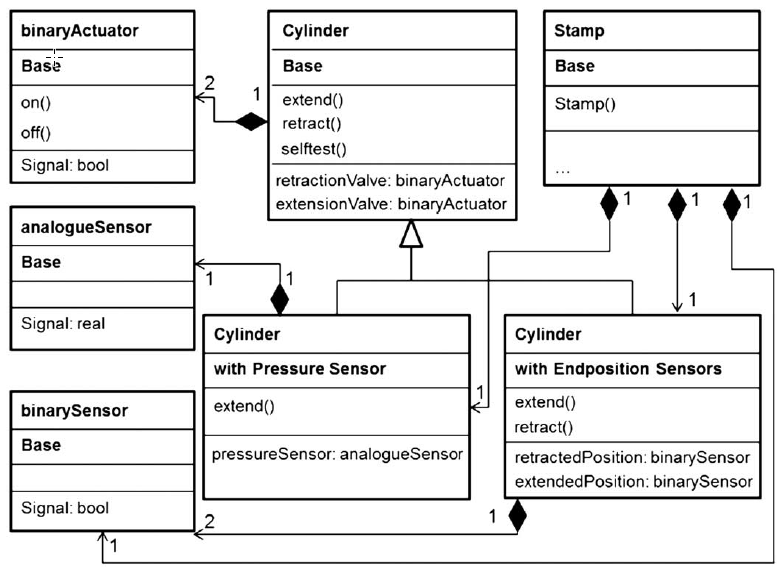
\includegraphics[width=\textwidth]{./Figures/modAT4rMS_struct.png}
		\caption{Structural definition of the press setup.}
		\label{fig:modAT_struct}
	\end{subfigure}
	\begin{subfigure}{\textwidth}
		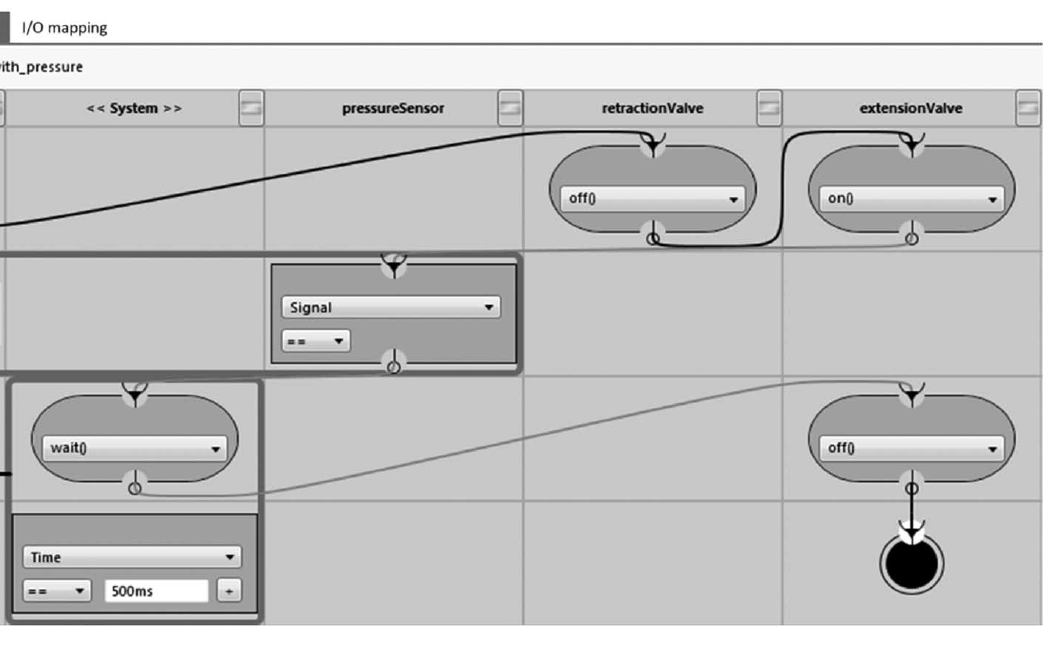
\includegraphics[width=\textwidth]{./Figures/modAT4rMS_beh.png}
		\caption{Behavioral definition of the stamp press.}
		\label{fig:modAT_beh}
	\end{subfigure}
	\caption[Example of a modAT4rMS specification for a two-cylinder press setup.]{Example of a modAT4rMS specification for a two-cylinder press setup.~\cite{Obermeier:2015aa}}
	\label{fig:modAT}
\end{figure}
The actuator would provide a extend and retreat function, whereas the pressure sensor would allow to define the applied pressure on the object.
The implementation of the functions must be defined at a later stage in modeling.
This structural definition uses adapted~\acrshort{acn:uml} class diagrams defined for plcML.
Secondly, the behavior of the components must be defined.
For this they use activity and state-charts that are defined for a certain module.
In a behavior definition for a module, the functions and attributes defined in the structure diagram are used.
They can be combined to form a state machine depending on different conditions.
In figure~\ref{fig:modAT_beh} an example of the behavior specification for the stamp press defined in~\ref{fig:modAT_struct} is shown.
The presented specification language is powerful as enables the developer to specify system behavior and structure in a clear and concise manner.
In terms of effectiveness, the approach covers many levels of abstraction and covers the full extent of a PLC's capability.
Additionally, the definition of the structure and behavior of a system can be translated into IEC 61131-3 code to directly run on a~\acrshort{acn:plc}.
This increases efficiency and reduces the number of errors while moving from the model to the code.
The transformation is described in detail in~\cite{WITSCH2015}.
\citeauthor{Obermeier:2015aa} conducted a study to investigate the impact the refinements have on user acceptance and efficiency.
They conclude that their refinements increase the usability and efficiency during development significantly compared to the pure plcML specification and slightly compared to the basic IEC 61131-3 languages.
In addition, they state that their method scales to larger project and more diverse teams in terms of experience.
This gives the method a good real-world applicability.

\citeauthor{6957399}~\cite{6957399} describes an automatic code generation algorithm for~\acrshort{acn:plc} from a~\acrshort{acn:sml} specification.
They use the~\acrshort{acn:sml} block diagram and the state-machine diagram to define the full system specification required for code generation.
To express the system structure, they redefine keywords from the SysML block diagram.
This gives the approach good real-world applicability with SysML being an established language that is widely used in the systems design industry.
It also requires less additional training and development tools than developing a brand-new specification method.
They allow to define a blocks input, outputs, global variables, different classes of organizational units and safe states.
\begin{figure}[h]
	\begin{subfigure}{0.5\textwidth}
		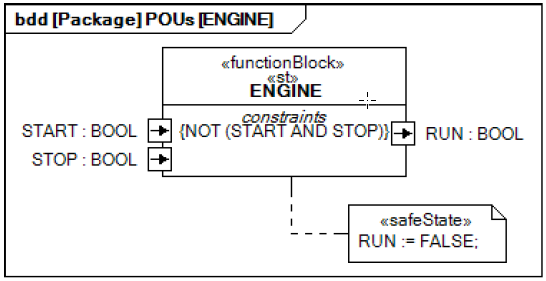
\includegraphics[width=\textwidth]{./Figures/sysml_bdd.png}
		\caption{Block description diagram for an engine unit.}
		\label{fig:sysml:bdd}
	\end{subfigure}
	\begin{subfigure}{0.5\textwidth}
		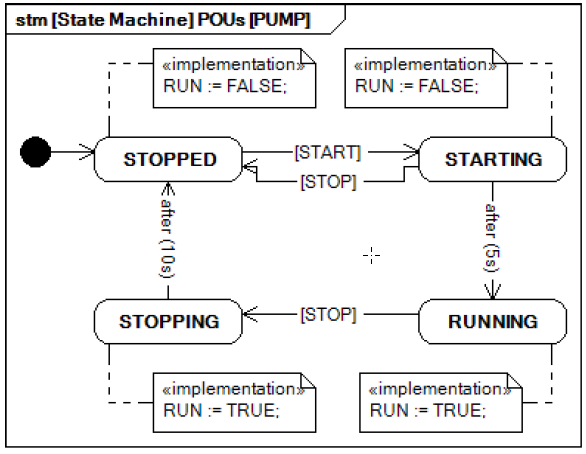
\includegraphics[width=\textwidth]{./Figures/sysml_stm.png}
		\caption{State machine for a pump unit.}
		\label{fig:sysml:stm}
	\end{subfigure}
	\caption[Example of a SysML specification for an engine and pump unit.]{Example of a SysML specification for an engine and pump unit.~\cite{6957399}}
\end{figure}
Figure~\ref{fig:sysml:bdd} shows a block definition diagram for an engine unit.
In this example the engine has two Boolean inputs, an invariant that both inputs cannot be true, and a single Boolean output.
In addition to the blocks, a state-machine based model of the block can also be specified.
This allows to generate a fully functional block instead of just the framework for it.
For every state,~\acrshort{acn:ST} code can be specified that is executed upon entry into the state.
A use case for this, is to assign variable values.
But this restricts the effectiveness of the approach slightly, as not all possibilities of behavior specification can be covered with this method.
When a process cannot be modeled with a state machine, the specification can only generate a framework and the developer must write the actual IEC 61131-3 code himself.
Figure~\ref{fig:sysml:stm} shows the state machine definition for a pump module.
The pump has the same block definition diagram then the engine shown in~\ref{fig:sysml:bdd}.
In the comment elements attached to the states, the ST code to run on state entry is defined.
They implement a template-based code generator that uses the previously specified models and generates a~\acrshort{acn:ST} code implementation of the model.
For this the model is converted into a series of ordered operations that must be executed in a PLC cycle.
Every operation derived from a state in the state machines and the block definitions is then mapped to ST code.
This procedure has the benefit of allowing round trip engineering as the generated code can be altered and re-transformed into the model if the edits don't alter the fundamental structure.
This has a significant impact on efficiency, real-world applicability and user acceptance as the development times can be reduced and its easier for a developer to work with the code as well as the model.

\subsubsection{Simulink}
\label{sec:sub:simulink}

Simulink\footnote{\url{https://de.mathworks.com/products/simulink.html}} is a graphical programming environment for developing, simulating and analyzing systems.
It covers many system domains through a large availability of toolboxes.
It is integrated in MathWorks MATLAB environment.
A Simulink diagram consists of blocks that are connected via signals.
The toolboxes contain many pre-defined blocks realizing a common behavior for a specific domain.
For example, the~\enquote{Discrete} library provides a discrete PID controller that can be used in a closed-feedback loop system.
Blocks can also be nested allowing the user to create sub-blocks, introducing abstraction levels to a system specification.
The considerable number of available blocks and the general architecture of the system make Simulink a highly effective specification language.
Its versatility and ease of use, while still being able to handle complex models, even for designing larger systems, are core to its success.
In addition to the model definition, Simulink provides a large portfolio of verification and validation methods.
The model can be discretely simulated to observe the systems behavior, static model analysis methods are available and generic test suits can be defined.
This allows for an extensive model debugging before the model is deployed on the actual production system or a prototype.
The workflow of designing, simulating and analyzing is effective and intuitive.
For these reasons Simulink is commonly used in control system design and model-driven system development.
As it is widely used, a transformation approach using Simulink has a good real-world applicability.

Simulink provides a toolbox\footnote{\url{https://de.mathworks.com/products/simulink-plc-coder.html}} to encode an existing model in the IEC 61131-3 language~\acrshort{acn:ST}, called \enquote{Simulink PLC Coder}.
It can transform a Simulink model with input, output and storage nodes as well as nested blocks into a valid ST code implementation that can be run on a PLC.
For this to work, the blocks must exclusively consist of logical or mathematical functions.
This makes the coder remarkably effective as most of the Simulink features can be ported to a PLC without additional effort.
Of course, this also increases the user acceptance and real-world applicability of the method.
To allow traceability between the transformed model and the Simulink model, the coder can generate a traceability report that shows where and how blocks are implemented in the generated code.
The coder implements a set of optimization algorithms to reduce the complexity and size of the resulting ST code.
\citeauthor{7535242}~\cite{7535242} describe a workflow using this~\enquote{Simulink PLC Coder} and the~\enquote{Simulink C Coder}\footnote{\url{https://de.mathworks.com/help/dsp/ug/generate-c-code-from-simulink-model.html}} to develop, verify and deploy a model created in Simulink on a PLC.
In addition to the auto-generation and verification of the code in Simulink they implement a workflow using a bound model checker for C.
This is required as Simulink does not provide a model checking algorithm for its models.
For the verification they transform the Simulink model to C code, which is then combined with other C code that was manually created.
This manually created C code, contains the assertions, invariants and model parameters in a format that is accessible for the model checker.
They then feed the C files in the~\acrfull{acn:cbmc}.
The checker runs the model an verifies the defined model invariants and parameters.
As this validates only model behavior, this result can be transferred to the Simulink model.
This allows for a deeper validation of the model than the other methods offered by Simulink.

\citeauthor{6489667}~\cite{6489667} compare different code generator approaches for Simulink models to PLC code.
Additionally, they develop their own code generator which transforms Simulink to~\acrfull{acn:CFC}, a non-standard language for PLC programming developed by Siemens.
They decided to use~\acrshort{acn:CFC}, as its graphical structure is close to the one used for Simulink models.
For ST based code generators this is not the case.
This increases user acceptance and efficiency as the transformed code can be read and understood easier.
Additionally, this feature permits re-transformation from the~\acrshort{acn:CFC} model to a Simulink model.
Hence, operations such as roundtrip engineering can be supported, which is more challenging with ST code.
This provides a major improvement in real-world applicability and efficiency over the previously investigated approach.
A problem with~\acrshort{acn:CFC} is that the supported features are differing widely between, different PLC environments.
This requires their code generator to generate function blocks differently for different PLC environments.
Such a restriction reduces the effectiveness and the real-world applicability significantly.
The dependency on the capabilities of the PLC environment make it hard to use the system compared to other platform independent approaches.

\subsubsection{GRAFCET}
\label{sec:sub:grafcet}

GRAFCET is a graphical modeling language allows the discrete modeling of control systems.
It was designed as a modeling language for the IEC 61131-3 implementation languages.
For this reason, it is a reasonable candidate for a code generation-based modeling approach.
The language uses a similar syntax and semantic to petri nets.
\begin{figure}[h]
	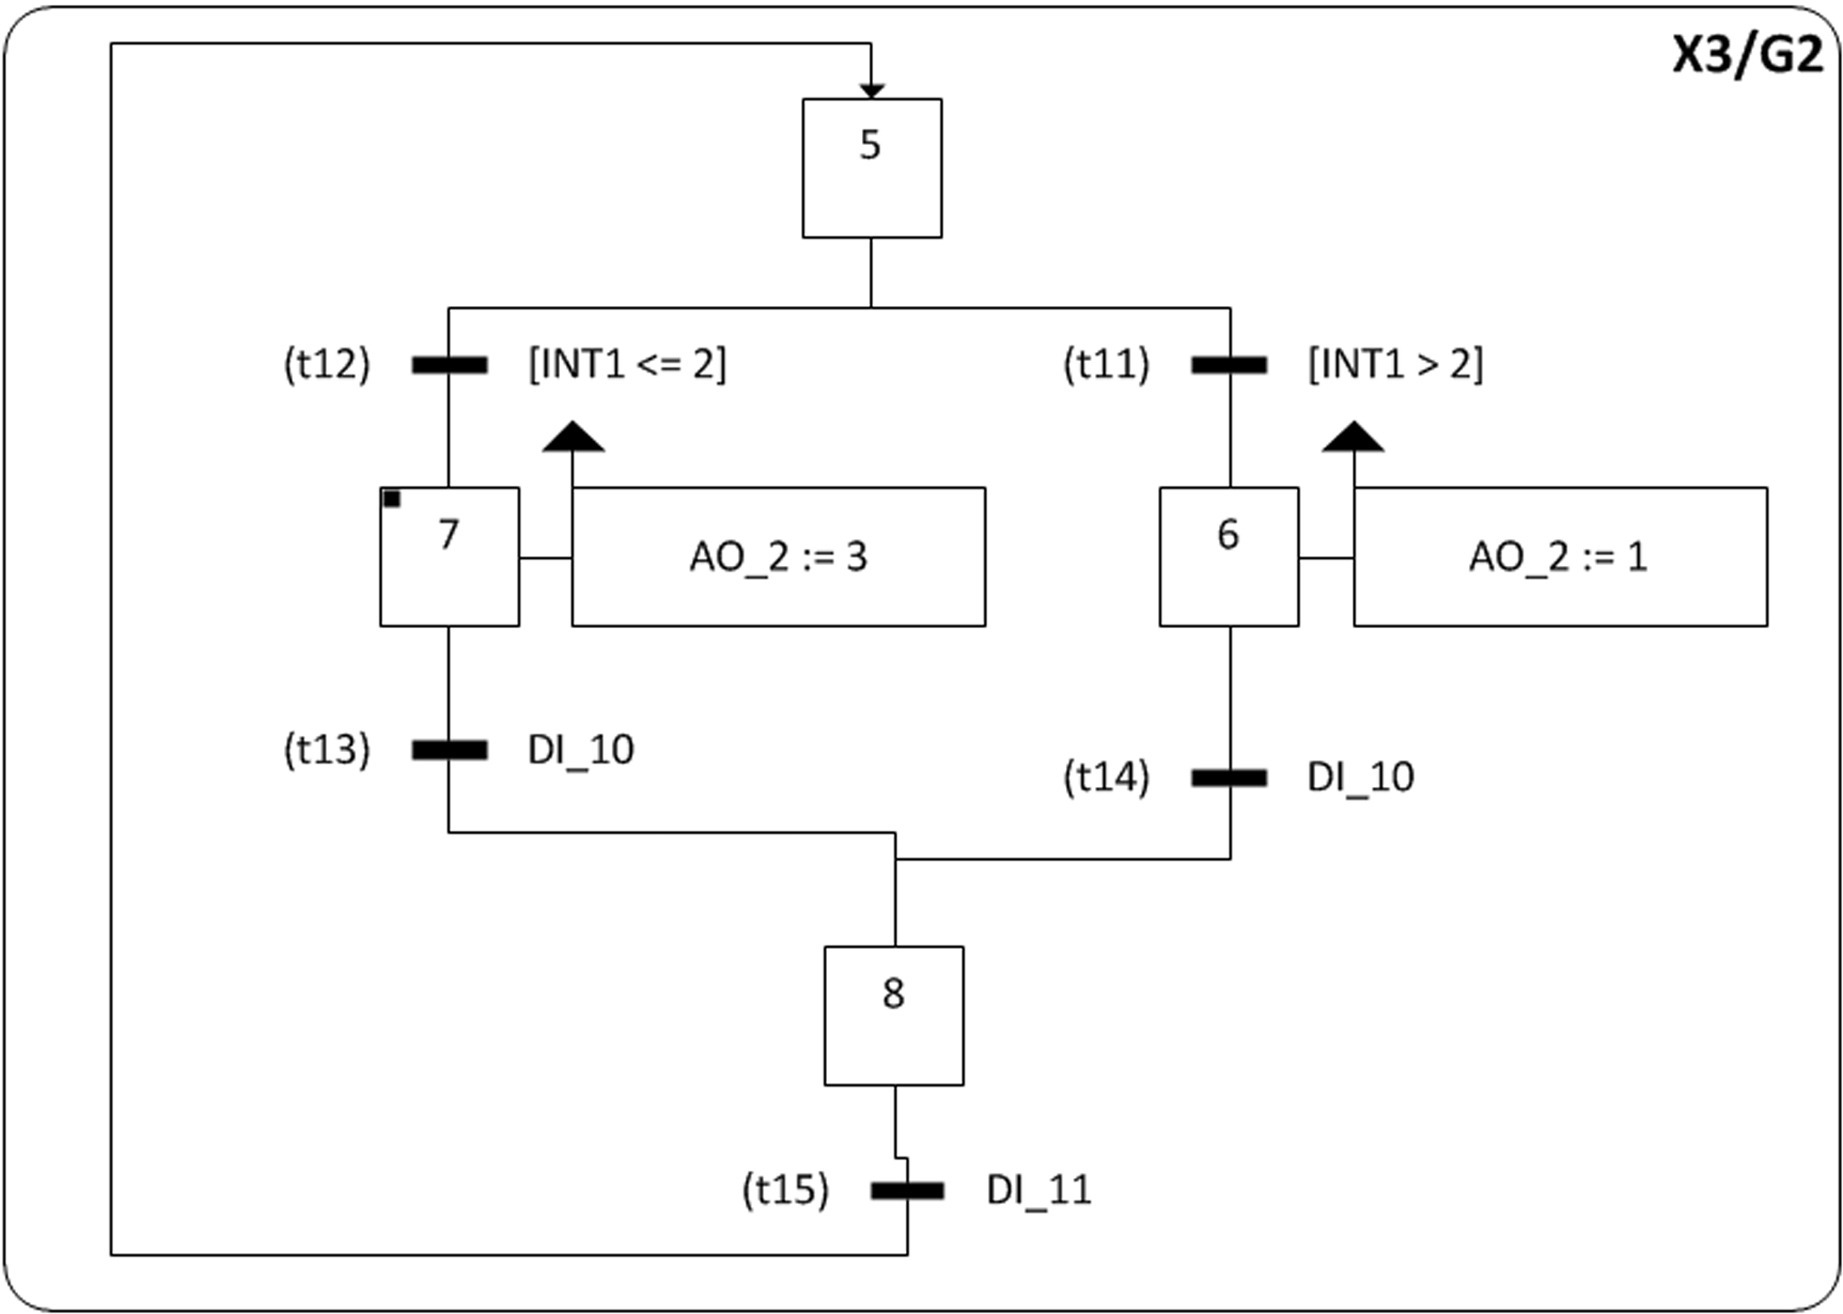
\includegraphics[width=\textwidth]{./Figures/grafcet_ex.jpg}
	\caption[Example of a GRAFCET specification.]{Example of a GRAFCET specification.~\cite{JULIUS2017173}}
	\label{fig:grafcet}
\end{figure}
Common elements are states, state transitions with attached conditions, sub-systems in states and forks of the control flow.
Figure~\ref{fig:grafcet} shows an example of a GRAFCET specification.
Here the sub-systems inside a state and the control flow constructs mentioned before can be recognized.
The full GRAFCET language specification is published under the IEC 60848 standard~\footnote{\url{https://webstore.iec.ch/publication/3684}}.
\citeauthor{JULIUS20191767}~\cite{JULIUS20191767, JULIUS2017173} present a ST source code generation algorithm from GRAFCET specifications.
In~\cite{JULIUS2017173} they present the generation algorithm but without supplying an implementation and addressing time and event constrains.
With~\cite{JULIUS20191767} they present an Eclipse EMF based editor including an implementation of the generation algorithm.
Additionally, time dependencies and events can be specified and handled.
Their code generation algorithm ensures that the exact semantics of the GRAFCET specification are transferred to the ST code.
For this they define a rule-based interpretation algorithm that simulates a GRAFCET execution in ST code.
In addition to ST code, they can also generate specifications for other PLC code formats like PLCOpenXML and Structured Control Language for Siemens platforms.
This gives their approach a wide range of target platforms increasing its real-world applicability.


%% ==============================
\subsubsection{PLCspecif}
\label{sec:sub:plfspecif}
%% ==============================

\citeauthor{7819191}~\cite{7819191, darvas2015syntax, darvas2015requirements, darvas2015formal, 10.1007/978-3-319-33693-0_32} define a~\acrshort{acn:dsl} for~\acrshort{acn:plc} behavior specification and system modeling called PLCSpecif.
They created the language to allow model driven development on a PLC without having problems with validation and verification.
Core goals were ease of use, formal verification capability and readability of the generated ST code.
PLCSpecif uses a composition of modules to describe the behavior of the control program.
Every module consists of three parts, input specification, core behavior specification and the output specification.
For the core behavior there are two types of Modules, Composite Modules, where the core describes a sequence of modules, and Leaf Modules, where the core is a single mealy machine.
To define the transitions in the mealy machine, events can be specified that are triggered when a logic formula using the input variables is evaluating true.
This model of a control program creates a big state machine from several submodules.
A pre-processing step is used to translate events and conditionals into transitions that use guard variables and active state variables.
Such a pre-processing is required to ensure that the transitions run correct and no errors such as infinite loops or non-determinism are present.
After this step, a SAT solver can verify the correctness of the  transitions by searching for directed cycles of non-event transitions or multiple transitions from one node with equivalent guards.
They use the mealy machine structure of the system to verify some general features like the absence of dead code or deadlock / livelock freeness.
Additionally, they support the specification of module invariants that can be checked on the final composite model.
In~\cite{10.1007/978-3-319-33693-0_32} they specify methods to transform existing PLC code to an intermediate model and compare this to an existing PLCSpecif specification.
They do this by using model equivalence or conformity checks.
To verify the code generated from PLCSpecif as described in~\cite{7819191} they use the same method than for legacy non generated code.
For code generation they use, a model to model transformation.
They transform states into variables or enums, and transitions are translated into IF-THEN blocks.
To fulfill the requirement of readable generated code, the first transform into an abstract ST representation and then use simplification algorithms to reduce the complexity of the code.
The abstract ST representation is then transformed into the actual ST code.
This also increases portability as some ST language features are not supported on all PLC platforms.
The correctness of the transformation is ensured as the structure that is implemented in ST is the transition graph that can be implemented directly.
There are no advanced transformations but just a plain model to text transformation with the same basic semantics.
